\documentclass[paper=a4, fontsize=11.5pt]{scrartcl}
\usepackage[T1]{fontenc}
\usepackage{fourier}
\usepackage{tabularx}
%\usepackage[english]{babel}															
\usepackage[english]{babel}
\usepackage{indentfirst}		% for indent
\usepackage[utf8]{inputenc}

\usepackage[protrusion=true,expansion=true]{microtype}	
\usepackage{amsmath,amsfonts,amsthm} % Math packages
\usepackage[pdftex]{graphicx}	
\usepackage{url, array}
\usepackage[num,abnt-repeated-author-omit=yes]{abntex2cite}


%%% Custom sectioning
\usepackage{sectsty}
\allsectionsfont{\centering \normalfont\scshape}


%%% Custom headers/footers (fancyhdr package)
\usepackage{fancyhdr}
\pagestyle{fancyplain}
\fancyhead{}											% No page header
\fancyfoot[L]{}											% Empty 
\fancyfoot[C]{}											% Empty
\fancyfoot[R]{\thepage}									% Pagenumbering
\renewcommand{\headrulewidth}{0pt}			% Remove header underlines
\renewcommand{\footrulewidth}{0pt}				% Remove footer underlines
\setlength{\headheight}{13.6pt}


%%% Equation and float numbering
\numberwithin{equation}{section}		% Equationnumbering: section.eq#
\numberwithin{figure}{section}			% Figurenumbering: section.fig#
\numberwithin{table}{section}				% Tablenumbering: section.tab#


%%% Maketitle metadata
\newcommand{\horrule}[1]{\rule{\linewidth}{#1}} 	% Horizontal rule

%\date{\today}

%%% Begin document
\begin{document}
		
{\flushleft\horrule{2pt}
\begin{center}
{
\includegraphics[height=0.09\textwidth]{Figs/logo_english.png}} 
\begin{tabular}{ m{1.8cm} m{10cm} m{1.8cm}}
\begin{center}
\end{center}
&
\begin{center} 
{\small
{Adrar University} \\
{Faculty of Science and Technology} \\
{Department of Mathematics and Computer Science}} \\

\end{center}
&

\begin{center}
\end{center}
\end{tabular}
\end{center}
\flushleft \horrule{2pt}\\[1cm]
}


\begin{center}

{
\huge  
Initiation to Research (Course) \\
\vspace{0.2cm}
2\textsuperscript{nd} Year Master (S3) \\
\vspace{0.2cm}
2020/2021}\\

\vspace{1cm}

{
\Huge   
\textbf{Multi-Agent Modeling the Spread of COVID-19 pandemic }}\\
\vspace{1cm}

%Domain: Mathematics and Computer Science \\
%Major: Informatics - Intelligent Systems \\
{
\Large
\textbf{Ould Miloud Ahmed \footnote{Email: ahmed.ouldmiloud@gmail.com}}}\\
\vspace{4.5cm}

{
\large
\textbf{Instructor: Dr. Abdelghani DAHOU \footnote{Email: dahou.abdghani@univ-adrar.edu.dz}}}\\
\today
\end{center}
\pagebreak
\tableofcontents
\pagebreak
\listoffigures
\pagebreak
\listoftables
\pagebreak
\doublespacing



\section{ Abstract}
\quad In this work we In this work we will use the concept of modeling and simulation to develop a Multi-Agent model combined with an existing mathematical model, which will describe the dynamics of the spread of the \emph{Covid-19} pandemic in our country \emph{Algeria}. The mathematical model used is inspired from the classic \emph{SEIR} Model and the Multi-Agent model contains five kinds of agent each one has a specific role: Person Agent, Medical Sector Agent, Laboratory Agent, Authority Agent. Finally, to test the scenarios, we will retrieve information on the number of cases with a confirmed \emph{Covid-19} infection based on the official reports of government institutes in Algeria (Algerian Ministry of Health 2020)
\section{Keywords}
\textmd {Covid-19, SEIR, Multi Agent, Pandemic ,Modeling, Simulation.}
\section{Introduction}
\quad Over December 2019, many cases of unknown pneumonia were detected in \emph{Wuhan},\emph{ Hube}i province, \emph{China}, due to a novel coronavirus \emph{Sars-cov-2}, called later \emph{Covid-19}. This pandemic has steadily spread in China  first, then to the other countries. In \emph{Algeria} the first case reported on February 25, 2020 was imported from \emph{Italy}, and then spread to other regions of the country very quickly with 139 cases confirmed until March 21, 2020[9], which forced the national government to put a plan and tools to fight against this new threat, so several scenarios were applied by the government.\\
\smallskip
\qquad As it is crucial to estimate the number of infections and predict the growth of the pandemic it is consequently important to model the spread of the pandemic in time in order to understand how the pandemic is spreading and predict its trajectory, also it makes possible to evaluate and modify the public health measures and inform our health system about then number of patients expected.\\
\smallskip
\qquad In this work we will use the concept of modeling and simulation to develop a multi-agent model combined with an existing mathematical model, which will describe the dynamics of the spread of the Covid-19 pandemic and evaluate possible scenarios to fight this pandemic.\\
To develop this model, we will use an existing deterministic mathematical model extracted from the classical \emph{ SEIR} model. The Multi-Agent system is composed of five kinds of agents: Person Agent, Medical Sector Agent, Laboratory Agent, Authority Agent and Evaluator Agent, each Agent has a specific role. To be able to test the scenarios, we will retrieve information on the number of cases with a confirmed COVID-19 infection based on the official reports of government institutes in Algeria \emph{ (Algerian Ministry of Health 2020)}.


\section{Related Works}
\quad Since the  \emph{WHO \footnote{World Health Organization}} declared the Covid-19 pandemic as an international public health emergency, several scientific works have been started, to investigate the dynamics of transmission of Covid19. Overall, the mathematical SEIR model represent the majority among those proposed in the literature \cite {kamrujjaman2020pandemic}\cite {godio2020seir}\cite {sardar2004assessment}\cite {ullah2020modeling}. Nevertheless, some articles with an agent-based model have also been proposed.\\
\smallskip
\qquad In the paper released by Giuseppe Antonio Nanna et al \cite{nanna2020multi}, the proposed Multi-Agent model improves the previous Multi-Agent approaches by adding a new set of features to control the pandemic during simulation to check how government strategies can influence the spread of the disease in Italy.\\
\smallskip
\qquad To get an idea about the components of the\emph{ MAS \footnote{Multi-Agents  System}} model to be developed to handle Covid-19 situations, we refer to the suggested model to simulate the dynamics of the Covid-19 epidemic and the epidemiological and economic effects of social distancing interventions in Brazil by Petrônio Cândido \cite{silva2020covid}. Also, Sharma, et al, used autonomous entities(agents), who work collaboratively to develop a Multi‑Agents system to Handle patients during the covid‑19 pandemic\cite{sharma2020multi}.\\
\smallskip
\qquad In the current work, we use a SEIR model with a MAS Components to simulate the dynamics of the spread of the Covid -19 pandemic and we perform analysis to some scenarios.
\section{Methodology/Research Methods}
\subsection{Epidemiological data: }
\quad We retrieved information on cases number with confirmed Covid-19 infection based on official reports from governmental institutes in Algeria (Algerian Ministry of Health 2020)\cite{hamidouche2020covid}.

\subsection{Mathematical model }

\quad In order to predict the transmission dynamics of Covid-19 we will use an existing deterministic mathematical model extracted from the classical SEIR model defined by the following differential equations :\\
\medskip
$^C D_t^\alpha S=\Delta - \frac{(v_1I_u + v_2I_r + v_3I_c)}{N}S - \mu S$\\
$^C D_t^\alpha A=\frac{(v_1I_u + v_2I_r + v_3I_c)}{N}S -( \sigma + \mu )A$\\
$^C D_t^\alpha I_u=\sigma (1 - \rho)A - (\mu + \gamma _{I_u }+ d_1) I_u$\\
$^C D_t^\alpha I_r=\sigma\rho A - (\delta_{I_r }+ \gamma _{I_r }+ \mu) I_r$\\
$^C D_t^\alpha I_c=\delta_{I_r }I_r - (\gamma _{I_c }+ \mu + d2) I_c$\\
$^C D_t^\alpha R=\gamma_{I_u }I_u + \gamma_{I_r }I_r + \gamma_{I_c }I_c - \mu R$\\
\medskip
The tables below show respectively the compartments and the parameters of the model
\begin{table}[h]
\centering
\begin{tabular}{cl}  
	\hline
	Compartment & Content\\
	\hline
	$S$  & Susceptible people\\
	$A$  & Asymptomatic people\\
	$I_u$  & Undetected infectious people\\
	$I_r$  & Detected infectious people\\
	$I_c$  & Critical infectious people\\
	\hline
\end{tabular}
\caption{The compartments of the model}
\label{tab:Table1}
\end{table}
\medskip
\begin{table}[!h]
\centering
\begin{tabular}{cl}  
	\hline
	Parameter & Description\\
	\hline
	$\Delta$ & Birth rate\\
	$\mu$ & Natural Death rate\\
	$v_1$  & Transmission rate of undetected people\\
	$v_2$  & Transmission rate of detected people\\
	$v_3$  & Transmission rate of critical people\\
	$d_1$  &  Infection induced death in $I_u$ class\\
	$d_2$  &  Infection induced death in $I_c$ class\\
	$\sigma$ & Incubation rate\\
	$\gamma_{I_u }$ &Recovery rate of undetected infectious people\\
	$\gamma_{I_r }$ &Recovery rate of detected infectious people\\
	$\gamma_{I_c }$ & Recovery rate of critical infectious people\\
	$\delta_{I_r }$ & Critical rate of detected infectious people\\ 
	\hline
\end{tabular}
\caption{Description of the parameters of the model}
\label{tab:Table2}
\end{table}
\\
\\
the different stages of transmission of Covid-19 into the compartments are represented as follows:
\begin{figure}[h]
	\centering
	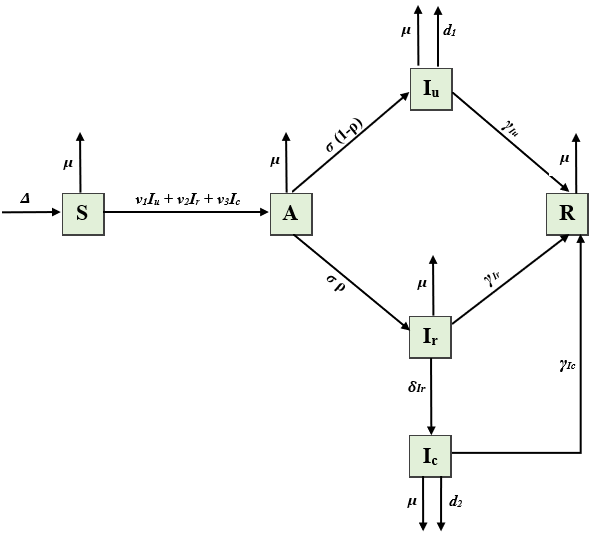
\includegraphics [width=0.95\linewidth]{ Figs/SEIR.png}
	\caption{Transmission of Covid-19 into the compartments}
	\label{Figure1}
\end{figure}

\subsection{Multi-Agents Model : }
\quad The Multi-Agent system is composed of five kinds of agents: Person Agent, Medical\_Sector Agent, Laboratory Agent, Authority Agent and Evaluator Agent, each agent has a specific role

\subsubsection{Person Agent}
\quad It's the main focus of our modeling it is a visible agent and mobile in the environments. His actions in the environment and interactions with other agents constitute the mechanism by which infections occur. It has a set of attributes that can be summarized as follows: age, gender, Type, chronically ill, color, function or sector of work.

\subsubsection{Laboratory Agent}
\quad The Laboratory Agents allowed to the Medical\_Sector Agent to know if the person agent is at first infected or not and later if he is recovered.

\subsubsection{Medical\_Sector Agent}
\quad In this work we will use the mathematical model described above, inspired by the SEIR model. The role of the Medical\_Sector Agent to put each Person Agent according to his health condition in the appropriate compartment, which means changing the type of the Person Agent and consequently its color in the interface, also it informs the Authority Agent about the number of Person Agents in each compartment.

\subsubsection{Authority Agent}
\quad The Authority agent make decisions about the protocols to follow, and modify the public health measures as he sees proper to decrease the spread of the epidemic. These decisions depend on Evaluator Agent and Medical\_Sector Agent informations.

\subsubsection{Evaluator Agent}
\quad The behavior of This agent depends on the chosen mathematical model its role is to evaluate results obtained by the decisions of the Agent Authority in other way it evaluates the results of our Multi-Agent model.

\section{Project Timeline}
\quad To achieve the aim of the project, we need to break it into several steps, which contain a set of tasks, each task has a specific schedule, as it is showing in the table below
\begin{table}[h]
\centering
\begin{tabular}{l|l|l|l}  
	\hline
	Step & Task & Begin date & End date \\
	\hline
	Reading& Literature research & 02/01/2021 & 22/01/2021\\
	                                                 & Literature review & 23/01/2021 & 05/02/2021\\
	\hline
	Developing& Choose a SEIR & 06/02/2021 & 12/02/2021\\
	                           & Design a MA model& 13/02/2021 & 26/02/2021\\
	                           & Coding & 27/02/2021 & 23/04/2021\\
	\hline
          Testing & Define scenarios & 24/04/2021 & 30/04/2021\\
					  & Review the results & 01/05/2021 & 07/05/2021\\
	                                             & Discuss the results & 08/05/2021 & 21/05/2021\\
	\hline
	Editing & Editing chapter 1 & 27/02/2021 & 05/03/2021 \\
				         & Editing chapter 2 & 13/03/2021 & 26/03/2021\\
	                                         & Editing chapter 3 (part1) & 10/04/2021 & 23/04/2021\\
				         & Editing chapter 3 (part2) & 08/05/2021 & 21/05/2021\\
	\hline
	
\end{tabular}
\caption{Tasks scheduling }
\label{tab:Table3}
\end{table}
\\
The project in the estimate requires 7 months and 2 weeks (224 days )to be completed sequentially, so we need to do some tasks in the same time as shown in the figure below:
\begin{figure}[!h]
	\centering
	\includegraphics [width=1.15\linewidth]{ Figs/Workflow.png}
	\caption{Workflow project}
	\label{Figure2}
\end{figure}
\pagebreak
\bibliographystyle{abnt-num}
\bibliography{ref}

\end{document}